%RK Klausur Loesungsversuch (faui2k13)
%compile with: latexmk -pdf $Dateinname
\documentclass{article}
\usepackage{amsmath}
\usepackage{hyperref}
%\usepackage{epsf}
%tkitz stuff
\usepackage{tikz}
\usepackage{listings}
\DeclareMathSizes{10}{10}{10}{10}
\setlength{\parindent}{0pt}
\title{Klausur M\"arz 2015 - L\"osungsvorschlag"}
\author{L\"o"sungen: faui2k13, Latexversion: Sheppy}
\begin{document}
	\maketitle
	\section{Allgemeine Fragen}
		\subsection{FTP}
			\textbf{a)}\\
				- Verschiedene TCP-Verbinndungen f\"ur Daten\"ubertragung und Streuerung/Befehle\\
				- Steuerung w\"ahrend Daten\"ubertragen m\"oglich\\
			\textbf{b)}\\
				- im Aktive Mode initialisiert der Server die Datenverbinndung zum Client nach Anfrage\\
				- im Passive Mode tun dies der Client selbst, das hat den Vorteil, dass die Firewall des Clients dann wahrscheinlich nicht die Verbinndung des Servers blockt\\
		\subsection{Adressierung}
			\textbf{a)}\\
				- ARP \\
				- BROTKAST an alle Ger\"ate mit der IP des gesuchten Ger\"ats als Payload\\
				- gesuchtes Ger\"at antwortet mit eigener MAC\\
				- Schicht 2 (Sicherungsschicht)\\
			\textbf{b)}\\
				- Nein, ARP ist bereits ein Gegenbeispiel\\
			\textbf{c)}\\
				Ja, da beide im gleichen Subnetz sind
				\begin{align*}
					&HostB\;00001010\;00000000\;000000|01\;00000100 \\
					&HostC\;00001010\;00000000\;000000|11\;00001000
				\end{align*}
				Teilnehmer: $(2^10)$-2 = 1022
			\textbf{d)}\\
				- Vorteil: Auch bitfehler im IP-Header k\"onnen erkannt werden\\
				- Nachteil: Verletzung des Schichtenprinzips
		\subsubsection{Leitungskodierung}
			\textbf{a)}\\
				- selbsttaktend: Empfänger kann Sendertakt aus Signal gewinnen \\
				- gleichstromfrei: kein Gleichanteil im elektrischen Signal \\
			\textbf{b)}\\\\
				\begin{tikzpicture}[xscale=2]
					\draw 	(0,0) -- (0.25,0) -- (0.25,0.5) -- (0.75,0.5) -- (0.75,0) -- (1,0) --
							(1,0.5) -- (1.25,0.5) -- (1.25,0) -- (1.5,0) -- (1.5,0.5) -- (1.75,0.5) --
							(1.75,0) -- (2.25,0) -- (2.25,0.5) -- (2.5,0.5) -- (2.5,0) -- (2.75,0) -- 
							(2.75,0.5) -- (3.25,0.5) -- (3.25,0) -- (3.5,0) -- (3.5,0.5) -- (3.75,0.5) -- 
							(3.75,0) -- (4,0);
				\end{tikzpicture}\\
				-\hspace{3mm}0\hspace{8mm}1\hspace{8.5mm}1\hspace{8mm}1\hspace{9mm}0\hspace{8mm}
				0\hspace{8mm}1\hspace{8mm}1 \;\;- \\
		\section{TCP}
		\subsection{Round-Trip-Time}
			\[ RTT = 2*d_{prop} + 10ms = 2*45ms+10ms = 100ms \]			
		\subsection{TCP Verlauf}
			$A->B: SYN, Seq=1, Ack=XX 									\\
			A<-B: SYN, ACK, Seq=XX+1, Ack=2 							\\
			A->B: ACK, Seq=2, Ack=XX+2 									\\
			\textbf{\textit{Verbindung erfolgreich aufgebaut}} 			\\
			A<-B: Data, Seq=XX+2, Ack=3 \hspace*{1cm}|\;\;CW = 1		\\
			A->B: ACK, Seq=3, Ack=XX+3									\\
			\textbf{\textit{BANG!}}										\\
			A<-B: Data, Seq=XX+3, Ack=4									\\
			A<-B: Data, Seq=XX+4, Ack=5 \hspace*{1cm}|\;\; CW = 2		\\
			\textbf{\textit{Demnach weiterer Verlauf nach tau:}}		\\
			A<-B: Data, Seq=XX+3, Ack=4 \hspace*{1cm}|\;\; CW = 1		\\
			A->B: ACK, Seq=4, Ack=XX+4									\\
			A<-B: Data, Seq=XX+4, Ack=5 \hspace*{1cm}|\;\; CW = 2		\\
			A<-B: Data, Seq=XX+5, Ack=6									\\
			A->B: ACK, Seq=5, Ack=XX+5									\\
			A->B: ACK, Seq=6, Ack=XX+6									\\
			$\\
			Nach dem 4. Paket wurden 5000 Bytes uebertragen.
		\subsection{Leistungsanalyse}
				$d_{prop} = 45ms$\\\\
				$d_{trans} = \frac{L}{R} = 1ms\;\;denn\;10\frac{MBit}{s} =
				10^6 \frac{Bit}{s} = 1250\frac{Byte}{s}$\\\\
				$\frac{O}{L} = \frac{5000}{1250} = 4$\;\;\;\;$t = 2RTT + 4*1ms + 4*45ms = 384 (mit\;RTT\;als\;100ms)$
		\newpage
		\section{Programieraufgabe TCP-FIN}
			\begin{lstlisting}[language=java]
public class TCPFIN extends base {
	final int FIN_WAIT_1 = 1;
	final int FIN_WAIT_2 = 2;
	final int CLOSING = 3;
	final int TIME_WAIT = 4;
	final int CLOSED = 5;

	int state;

	void close() throws IOException {
		state = FIN_WAIT_1;
		send(FIN);
	}

	void receive(int flag) throws IOException {
		if (flag == FIN) {
			if (state == FIN_WAIT_1) {
				state = CLOSING;
			} else if (state == FIN_WAIT_2) {
				state = TIME_WAIT;
				startTimer();
			}
			send(ACK);
		} else if (flag == ACK) {
			if (state == FIN_WAIT_1) {
				state = FIN_WAIT_2;
			} else if (state == CLOSING) {
				state = TIME_WAIT;
				startTimer();
			}
		}
	}

	void timeout() throws WrongStateException {
		if (state != TIME_WAIT) {
			throw new WrongStateException();
		}
		state = CLOSED;
	}
}
\end{lstlisting}
\newpage
%unformated codeblock end
	\section{Routingverfahren}
		\subsection{Routingverfahren}
			\subsubsection{Darstellung}
				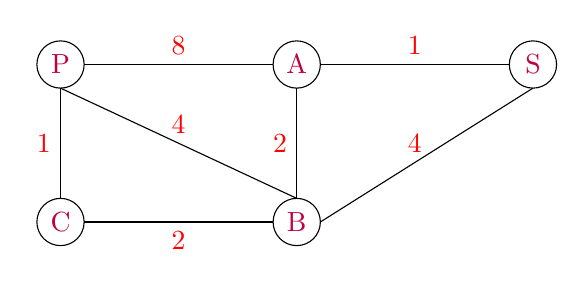
\begin{tikzpicture}
					%Knoten
					\draw(0,2) circle [radius=0.3];
					\draw(3,2) circle [radius=0.3];
					\draw(6,2) circle [radius=0.3];
					\draw(0,0) circle [radius=0.3];
					\draw(3,0) circle [radius=0.3];
					%Beschriftung Knoten
					\node[purple] at (0,2) {P};
					\node[purple] at (3,2) {A};
					\node[purple] at (6,2) {S};
					\node[purple] at (0,0) {C};
					\node[purple] at (3,0) {B};
					%Linien
					\draw (0.3,0) -- (2.7,0);
					\draw (0,0.3) -- (0,1.7);
					\draw (0.3,2) -- (2.7,2);
					\draw (3,0.3) -- (3,1.7);
					\draw (3.3,2) -- (5.7,2);
					\draw (3.3,0) -- (6,1.7);
					\draw (3,0.3) -- (0,1.7);
					%Beschriftungen Linien
					\node [left,red] at (0,1) {1};
					\node [above,red] at (1.5,2) {8};
					\node [above,red] at (1.5,1) {4};
					\node [below,red] at (1.5,0) {2};
					\node [left,red] at (3,1) {2};
					\node [red] at (4.5,1) {4};
					\node [above,red] at (4.5,2) {1};
				\end{tikzpicture}
			\subsubsection{Minimal aufspannender Baum}
				\begin{tabular}{| l | c | c | c | c | c |}
																								\hline
					N'		&	D(A),p(A)	&	D(B),p(B)	&	D(C),p(C)	&	D(P),p(P) 	\\ \hline
					S		&	1S	&		4S		&				&				  		\\ \hline
					SA		&	1S	&		3A		&				&	9A					\\ \hline
					SAB		&	1S	&		3A		&	5B			&	7B					\\ \hline
					SABC	&	1S	&		3A		&	5B			&	6C					\\ \hline
				\end{tabular}
			\subsection{Medienzugriff}
				\textbf{a)}\\ \\
					\begin{tabular}{|l|l|l|}
						\hline
						Zeit (in Bit-Zeiten)	&	Ereignis			& Erkl\"a"rung (nicht gefordert)	\\ \hline
						t = 0		&	A und B beginnen das Senden		&									\\ \hline
						t = 225 	&	A und B erkennen Kollision		&	$+=d_{prop}$					\\ \hline
						t = 273		&	Ende des Jam-Signals			&	$+=d_{jam}$						\\ \hline
						t = 498		&	letztes Bit kommt zu A			&	$+=d_{prop}$					\\ \hline
						t = 594		&	A beginnt mit \"U"bertragung	&	$+=d_{wait}$					\\ \hline
						t = 785		&	B \"u"berprüft ob Kanal frei ist&	$273+d_{back}$ Kanal-\"Uberpr\"ufung von 785-881	\\ \hline
						t = 1427	&	B beginn mit \"Ubertragung"		&	$1331$ (letztes Bit von a) + $96 d_{wait}$			\\ \hline
					\end{tabular}\\ \\ \\
				\textbf{b)}\\
					Nein denn Rahmengr\"osse $<=$ Backoffgr\"osse" und ein Konten geht immer in Backoff mit Faktor 1 und der andere mit 0.
					\\\\\\
					
	\begin{small}
		Diese Sammlung bassiert auf dem RK L\"osungspad des faui2k13 (\url{https://pad.stuve.fau.de/p/RK}) und enthält möglicherweise Fehler!
	\end{small}			
\end{document}
